\chapter{Lezione 4 - Architettura di Enterprise Resource Planning System}

Benvenuti a questa nuova lezione architettura di un enterprise resource planning system.
Tratteremo in questa lezione la parte che riguarda la gestione delle informazioni.
Gli argomenti che tratteremo sono lo schema dell'architettura, i principi fondativi di un enterprise resource planning system e la base delle informazioni, come le informazioni vengono gestite.

Argomenti trattati:

\FloatBarrier
\begin{figure}[H]
  \centering
  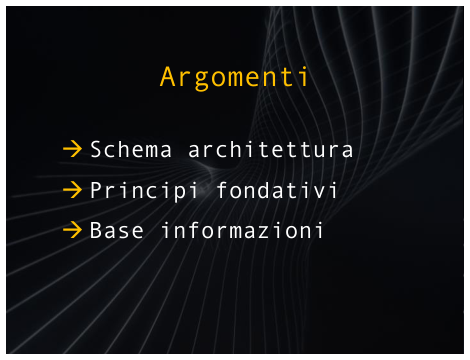
\includegraphics[width=0.50\textwidth,
                    trim=40 100 40 60, % L B R T
                    clip]
                    {images/Lez04_p01_fig_02}
  % \caption{Sommario}
  % \label{fig:Lez15_p06_fig_02}
\end{figure}
\FloatBarrier
\noindent

Ma vediamo innanzitutto il primo argomento, schema dell'architettura, e lo vedremo in una maniera molto sintetica, il massimo della sintesi.

\FloatBarrier
\begin{figure}[H]
  \centering
  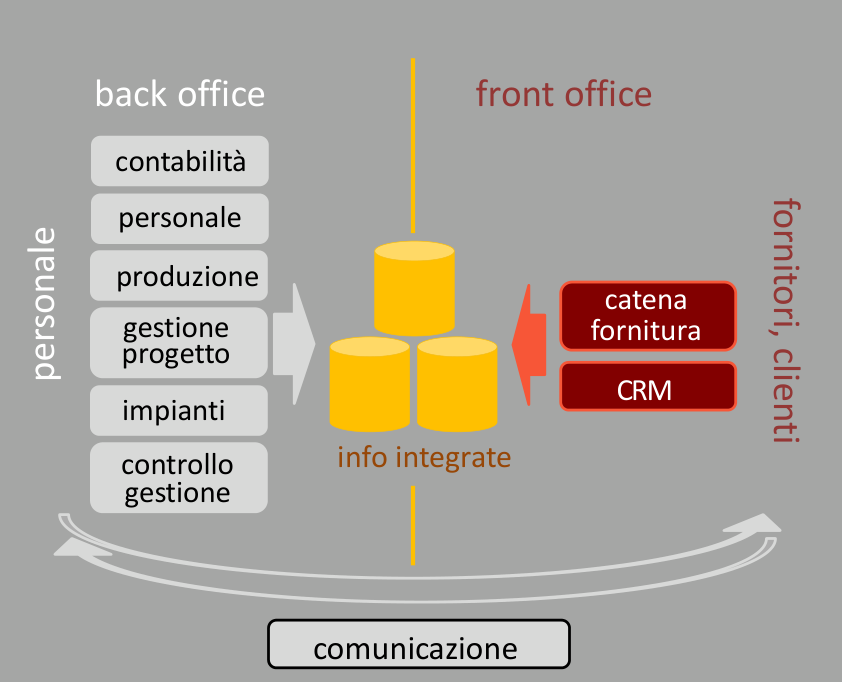
\includegraphics[width=0.50\textwidth,
                    trim=40 80 40 40, % L B R T
                    clip]
                    {images/Lez04_p01_fig_04}
  % \caption{Sommario}
  % \label{fig:Lez15_p06_fig_02}
\end{figure}
\FloatBarrier
\noindent

Vediamo lo schema dell'architettura di un enterprise resource planning.
Innanzitutto vediamo che individua due parti, il front-office che è la parte di un'organizzazione fornita del sistema che è interfacciata, interagisce con i fornitori e clienti.
Il front-office è quindi la parte dell'organizzazione che ha rapporti con l'esterno, che siano appunto gli acquirenti o che siano gli stakeholder o chi sostiene la catena di produzione.

Dall'altra parte abbiamo il back-office che include tutti gli uffici, i dipartimenti, l'organizzazione della impresa per sostenere i rapporti, le funzioni che vengono offerte all'esterno.
Il back-office offre, come abbiamo visto, funzionalità per gestire la contabilità, per gestire le risorse personali, per gestire la produzione, la gestione del progetto, il monitoraggio, la manutenzione degli impianti e il controllo di gestione.
Quindi un modulo o una funzionalità trasversale per il buon funzionamento, per la corretta gestione di tutti i moduli.

Le informazioni sono integrate, gestione integrata delle informazioni non significa necessariamente che le informazioni siano centralizzate anche se questo semplifica molto il lavoro ma a volte non ottimizza in quanto molti archivi, in questo caso, vengono mostrati icone di tre archivi, ma i tre archivi possono non essere mantenuti, possono non essere creati dalla stessa organizzazione, quindi essere centralizzati, ma da amministrazioni, organizzazioni differenti, quindi essere tre archivi remoti, quindi l'organizzazione si affida a una base di dati distribuita, l'importante è che la gestione, il controllo venga in qualche modo centralizzato nella organizzazione, cioè l'organizzazione si renda responsabile della corretto mantenimento di queste basi di dati.
Queste basi di dati vengono nutrite, alimentate, generate dall'acquisizione di dati esterni ma anche sostengono e vengono alimentate dai dati interni.
Basta pensare all'attività commerciale, all'attività del personale, di nuove acquisizioni di personale, costi del personale, nuovi prodotti realizzati e derogati.

Gli strumenti per la comunicazione servono sia all'interazione con il mondo esterno, quindi le comunicazioni con i fornitori, ma anche la fidelizzazione, l'attrazione dei clienti, attività di marketing, la fidelizzazione dei clienti, customer relationship management, sia anche la comunicazione all'interno del personale, quindi la comunicazione che avviene nel back office per l'interattività tra il personale interno all'azienda, ma anche sistemi di comunicazione per la corretta integrazione delle informazioni.
Quindi un'interoperabilità diciamo della parte statica del sistema e il trasferimento corretto delle informazioni.

Consideriamo questo argomento molto sinteticamente affrontato ma risolto e vi propongo due spunti di riflessione: focalizzate un ERPS, un sistema per la gestione delle risorse specifico per il vostro ambito lavorativo o formativo, quindi per l'ambito dove svolgete la vostra attività lavorativa o per l'università o la scuola che attualmente frequentate.

Un secondo spunto che gradisco proporvi è quali strumenti di comunicazione sono necessari tra il front office e il back office?
Quindi dovete individuare qual è il front office, quindi quali sono considerati gli elementi esterni all'organizzazione che usate di riferimento e quali interni.
Quindi lo spunto si riferisce a quali sono gli strumenti di comunicazione che secondo voi sono necessari al buon funzionamento dei rapporti, della comunicazione o dell'interattività tra interno e esterno dell'organizzazione.

\section{Principi formativi}

Passiamo ora, passiamo quindi ai principi fondativi dello sviluppo, della buona gestione, buona progettazione di un enterprise resource planning system.


\FloatBarrier
\begin{figure}[H]
  \centering
  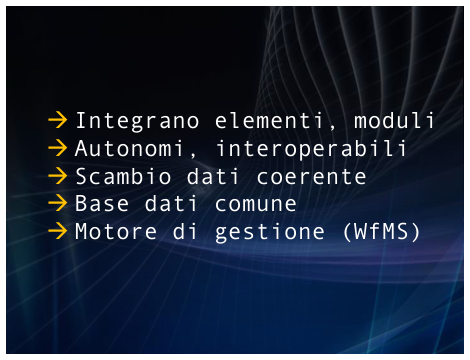
\includegraphics[width=0.50\textwidth,
                    trim=40 80 20 80, % L B R T
                    clip]
                    {images/Lez04_p02_fig_02}
  % \caption{Sommario}
  % \label{fig:Lez15_p06_fig_02}
\end{figure}
\FloatBarrier
\noindent


Il primo principio fondativo di un enterprise resource planning, come abbiamo visto, è l'integrazione degli elementi o moduli.
Tutte le funzionalità offerte per la gestione dell'impresa sono sostenuti da moduli specifici che devono essere integrati, ma oltre all'integrazione è richiesta l'autonomia e l'interoperabilità.

L'autonomia nel senso che ogni modulo deve contenere le funzionalità, gli elementi tecnologici realizzativi e le informazioni necessari al suo funzionamento e l'interoperabilità perché deve poter comunicare e scambiare dati con tutti gli elementi, quindi gli altri moduli, che compongono il sistema.

Inoltre lo scambio di dati coerente, tutti i moduli dovranno acquisire informazioni e poterle scambiare in maniera corretta e coerente col tipo di attività che stanno sostenendo.

La base di dati è comune, non è una base di dati centralizzata, ma comune nel senso che la gestione, come abbiamo visto, deve essere coordinata, deve essere allineata conforme agli obiettivi e alle attività comuni che sono svolte per sostenere l'impresa.

Infine è auspicabile anche un motore di gestione di flussi di lavoro per la pianificazione e per il controllo gestionale delle attività, dei processi interni all'organizzazione.

\subsection{Interoperabilità}

\FloatBarrier
\begin{figure}[H]
  \centering
  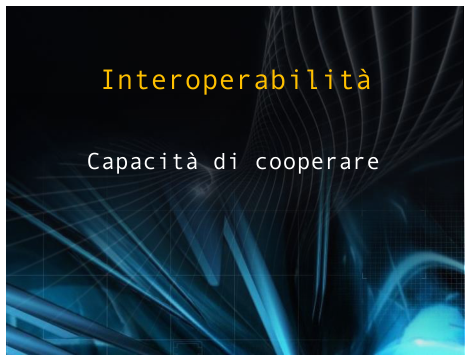
\includegraphics[width=0.50\textwidth,
                    trim=40 140 20 60, % L B R T
                    clip]
                    {images/Lez04_p02_fig_03}
  % \caption{Sommario}
  % \label{fig:Lez15_p06_fig_02}
\end{figure}
\FloatBarrier
\noindent


Il primo dei valori che sostengono questi principi fondanti è l'interoperabilità.

\FloatBarrier
\begin{figure}[H]
  \centering
  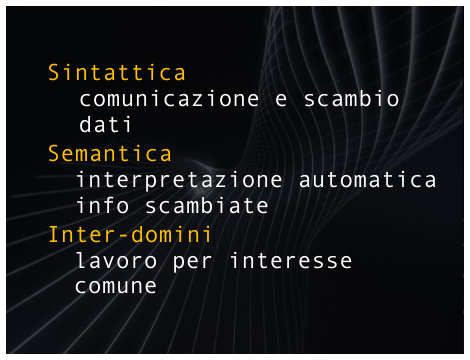
\includegraphics[width=0.50\textwidth,
                    trim=40 40 20 60, % L B R T
                    clip]
                    {images/Lez04_p02_fig_04}
  % \caption{Sommario}
  % \label{fig:Lez15_p06_fig_02}
\end{figure}
\FloatBarrier
\noindent

Interoperabilità significa, in maniera molto sintetica, la capacità di cooperare, ma l'interoperabilità è più strutturata, vi è un tipo di interoperabilità sintattica che si riferisce alla comunicazione e allo scambio dei dati.
La comunicazione e lo scambio dei dati, quindi i vari moduli, ma anche le varie persone, perché un'accezione più generale della interoperabilità coinvolge non solo gli elementi software, quindi i moduli, ma anche elementi sociali, politici, organizzativi, quindi elementi umani, funzioni svolte da risorse umane nell'ambito dell'organizzazione.
Ma tornando ai tipi di interoperabilità, il tipo di interoperabilità sintattica si riferisce allora alla comunicazione e allo scambio dei dati.
I dati devono essere scambiati in maniera corretta, in maniera non ambigua, sia tra i moduli, sia tra le persone, sia le persone devono essere in grado di interagire con il sistema in maniera coerente.

L'interoperabilità semantica riguarda l'interpretazione delle informazioni ricevute.
Le informazioni quando sono scambiate, se non sono interpretate allo stesso modo da chi le manda e da chi le riceve, sono inutili.
Per questo servono protocolli di intesa piuttosto che non strumenti per un'intesa comune come tesauri o in situazioni più complesse vengono utilizzate delle ontologie.
Molto spesso vengono utilizzati dei cataloghi, dei registri per l'organizzazione, la definizione dei metadati, quindi dei dati che descrivono le informazioni che abbiamo archiviate.

Il terzo tipo di interoperabilità è l'interoperabilità interdomini che riguarda il lavoro di interesse comune quando più organizzazioni possono essere anche imprese differenti o reparti della stessa impresa ma che hanno obiettivi specifici diversi, devono lavorare, si trovano a lavorare insieme, quindi a interoperare, hanno bisogno di una possibilità di intesa, un protocollo di comportamento che permetta di svolgere le rispettive autonome attività sempre in maniera coerente e convergente verso i comuni obiettivi.

\FloatBarrier
\begin{figure}[H]
  \centering
  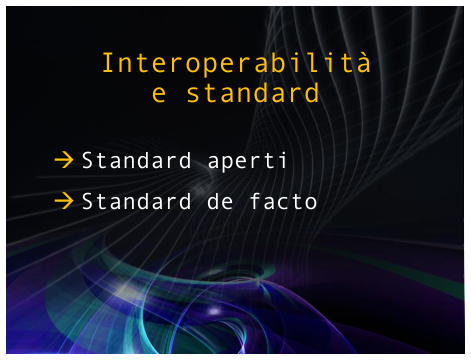
\includegraphics[width=0.50\textwidth,
                    trim=40 120 20 40, % L B R T
                    clip]
                    {images/Lez04_p02_fig_05}
  % \caption{Sommario}
  % \label{fig:Lez15_p06_fig_02}
\end{figure}
\FloatBarrier
\noindent
%%%%%%%%%%%%%%%%%%%%%%%%%%%%%%%%%%%%%%%%%%%%%%%%%%%%%%%%%%%%%%%%%%%%%%%%%%%
Un capitolo molto importante nell'interoperabilità è quello degli standard.
Vi sono due tipi di standard per l'interoperabilità standard aperti.
Gli standard aperti sono definiti, lasciatemi dire, a tavolino.
Organizzazioni rilevanti di un settore si riuniscono e i rappresentanti attorno a questo tavolo definiscono le regole che devono rispettare, i protocolli che devono rispettare tutti coloro che si muoveranno, agiranno, svilupperanno soluzioni e proposte in un certo settore, quindi diciamo sono standard predefiniti.

Poi ci sono gli standard de facto.
Gli standard de facto sono standard che hanno conquistato la loro posizione di riferimento sul campo.
Sono dovuti alla grande diffusione di uno strumento, alla grande diffusione di un'abitudine che di fatto diventa uno standard, diventa un riferimento condiviso, quindi non predefinito e in qualche maniera proposto o fatto adottare, fatto assimilare dalla comunità, ma al contrario, degli strumenti vengono utilizzati, dei modi di comportamento vengono utilizzati in maniera così diffusa che diventano degli standard.
Vi propongo alla fine di questo argomento uno spunto di riflessione.
Provate a individuare degli esempi di interoperabilità sintattica, semantica o interdomini, quindi degli esempi di interoperabilità dei tre tipi differenti che abbiamo definito.

\subsection{Base informazioni}

\FloatBarrier
\begin{figure}[H]
  \centering
  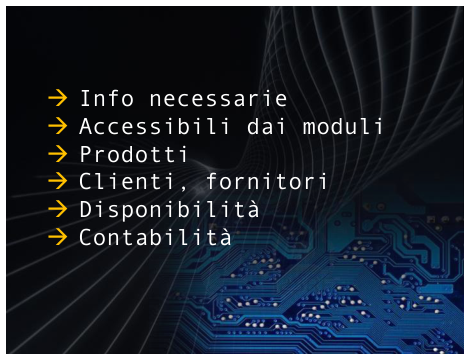
\includegraphics[width=0.50\textwidth,
                    trim=40 80 20 60, % L B R T
                    clip]
                    {images/Lez04_p03_fig_02}
  % \caption{Sommario}
  % \label{fig:Lez15_p06_fig_02}
\end{figure}
\FloatBarrier
\noindent

Vediamo ora la base delle informazioni, le caratteristiche delle base di informazioni di un enterprise resource planning system.
La base delle informazioni contiene solo le informazioni necessarie, quindi le informazioni necessarie in più i sistemi dovranno fornire, come vedremo e lo ripeteremo quando affronteremo l'argomento dei diversi tipi di sistemi per la gestione delle informazioni, devono evitare la ridondanza delle informazioni, quindi che le informazioni siano solo necessare e anche non ripetute.
Inoltre le informazioni devono essere accessibili da tutti i moduli che compongono il sistema.
Le informazioni forniscono o meglio una buona parte delle informazioni che sono contenute nella base informativa, nel database condiviso, e riguardano i prodotti.
I prodotti vuol dire che i dati forniscono informazioni riguardanti le denominazioni dei prodotti, i tipi, le materie prime costituenti, la capacità di produzione e la quantità.
Inoltre vi sono dati che riguardano i clienti e i fornitori, quindi gli ordini, le consegne effettuate, il catalogo dei fornitori.
Il catalogo dei fornitori è un registro piuttosto complesso che contiene tutti i dati amministrativi, i dati finanziari dei vari stakeholder, dei vari fornitori con cui un'organizzazione ha a che vedere.

Inoltre la disponibilità soprattutto dei prodotti in termini di durata o eventualmente in termini di consegna, nel caso di prodotti disponibili in potenzialità, ordinati ma non ancora consegnati.

Infine la contabilità, quindi tutte le informazioni che riguardano la contabilità, sia gli acquisti sia i pagamenti dovuti.

\FloatBarrier
\begin{figure}[H]
  \centering
  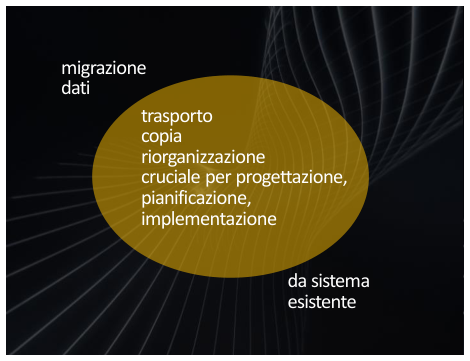
\includegraphics[width=0.50\textwidth,
                    trim=40 40 20 40, % L B R T
                    clip]
                    {images/Lez04_p03_fig_03}
  % \caption{Sommario}
  % \label{fig:Lez15_p06_fig_02}
\end{figure}
\FloatBarrier
\noindent

Un aspetto molto, molto importante, fondante, riguardante le basi informative riguarda la migrazione dei dati.
Un sistema informativo così complesso come un Enterprise Resource Planning abbiamo visto ha un uso in un'organizzazione che dura molto tempo, può essere sottoposto a diverse versioni, a diversi aggiornamenti, questo significa che in ogni versione, ogni cambiamento del software o delle strutture o delle risorse fisiche che vengono utilizzate, quindi non le risorse fisiche che vengono utilizzate, può rendersi necessaria una migrazione di dati dal sistema esistente al nuovo sistema.
Queste sono attività molto lunghe, costose in termini di tempo e di impegno lavorativo diffuso, perché le informazioni devono essere trasportate, quindi cambiate di formato dall'attuale sistema esistente a quello futuro, copiate, eventualmente riorganizzate se noi acquisiamo un sistema di base per l'archiviazione delle informazioni differenti.
Queste attività come dicevo sono molto costose, ma sono cruciali per la progettazione dell'attività di un'organizzazione, per la pianificazione e per l'implementazione di tutti i sistemi tecnologici che si basano sulle informazioni aziendali.

\FloatBarrier
\begin{figure}[H]
  \centering
  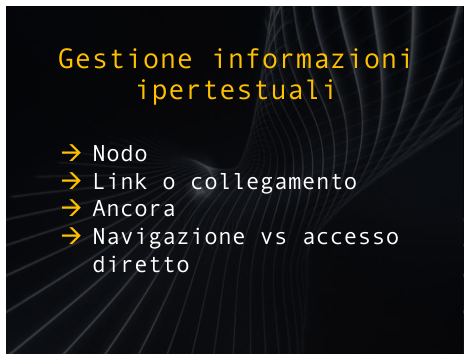
\includegraphics[width=0.50\textwidth,
                    trim=40 40 20 40, % L B R T
                    clip]
                    {images/Lez04_p03_fig_04}
  % \caption{Sommario}
  % \label{fig:Lez15_p06_fig_02}
\end{figure}
\FloatBarrier
\noindent

Vi sono diversi tipi di informazioni che costituiscono la base informativa di un'impresa.
Il primo tipo sono le informazioni ipertestuali.
Le informazioni ipertestuali nascono dagli ipertesti, dai famigiarati ipertesti, la cui ideazione risale ancora, ricordo, al 1945, non che siano stati costruiti i primi ipertesti informatici, ma l'idea della struttura ipertestuale nacque in quel periodo.
Autore di quest'idea fu Vannevar Bush, un consigliere governativo degli Stati Uniti.

Una struttura ipertestuale è composta di nodi.
I nodi sono gli elementi informativi e i frammenti di documento che vengono collegati da link, collegamenti che possono essere sintattici, ma in genere sono collegamenti semantici.
Quindi due nodi sono collegati tra di loro, dal progettista e dell'implementatore, se hanno un legame semantico, legame di senso o un legame dettaglio, se il nodo successivo è un approfondimento o un'alternativa.

Ipertesti e le strutture ipertestuali sono basate sull'uso delle ancore.
L'ancora suggerisce anche la parola stessa, sono quelle parti di un nodo attive.
Quindi quelle parti di un nodo attive sono quelle parti di un nodo che sono visibili, manifestano una possibilità di approfondimento, sono quelle parti di un nodo che fungono da aggancio a un nodo successivo, a un nodo di approfondimento o di dettaglio.

Il tipo di ricerca di informazioni in un ambito ipertestuale, in una struttura ipertestuale, è la navigazione, non l'accesso diretto.
L'accesso diretto è l'accesso effettuato o la ricerca effettuata a fronte di una interrogazione, cioè a fronte di un tipo di informazione, di una informazione, di una necessità informativa da parte dell'utente che viene descritta a priori in un'interrogazione e vengono così risolte da quello che è chiamato il motore di ricerca.
In un ipertesto invece si naviga, si entra nell'ipertesto e si cercano informazioni percorrendo i collegamenti tra un nodo e l'altro, selezionando le informazioni rilevanti.

\FloatBarrier
\begin{figure}[H]
  \centering
  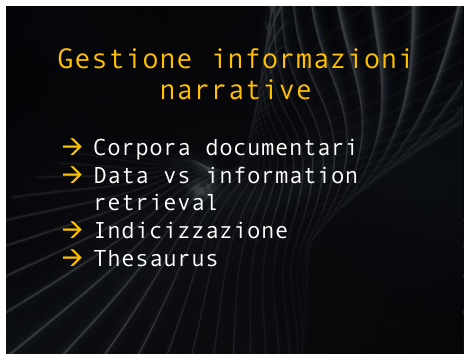
\includegraphics[width=0.50\textwidth,
                    trim=40 60 20 40, % L B R T
                    clip]
                    {images/Lez04_p03_fig_05}
  % \caption{Sommario}
  % \label{fig:Lez15_p06_fig_02}
\end{figure}
\FloatBarrier
\noindent

Un secondo tipo di informazioni sono le informazioni narrative, riguardano i corpora documentari, quindi insiemi di documenti rilevanti e coprenti, considerati esaustivi per un certo settore, un certo argomento, un certo tema.

Vi è una differenza da porre tra ricerca per dati o data retrieval e information retrieval, perché con data retrieval si fa riferimento a una ricerca precisa, cerco dei dati, voglio i documenti o voglio i record che esattamente rispondono alla mia descrizione di dato, contengono esattamente quel dato, vengono utilizzati per ricerche numeriche, per ricerche per cognome, codice fiscale o identificativi di altro genere.

Nel caso delle information retrieval invece le informazioni sono rilevanti per il significato, quindi io cerco una parola per il significato che porta, per me è rilevante anche un documento o può essere rilevante o interessante un documento che contiene informazioni sullo stesso ambito, informazioni con lo stesso significato o con un significato analogo.

Attività rilevante per la gestione delle informazioni narrative, quindi è l'indicizzazione, vuol dire che i documenti vengono trattati, vengono elaborati per produrre delle descrizioni sintetiche di quelli che sono i veri argomenti, i veri argomenti semantici che li rappresentano.
Uno strumento a supporto dell'indicizzazione e poi della risoluzione delle ricerche dirette, quindi per la risoluzione delle interrogazioni sono i Thesaurus.
I Thesaurus sono insieme strutturati di termini, strutturati in classi, i termini non hanno un valore sintattico ma hanno valore per il loro significato.

Le classi sono classi semantiche, possono essere classi di significato ma generalmente sono classi tematiche.
Tematiche cioè contengono i termini che riferiscono concetti che fanno parte dello stesso tema in interesse.

I thesaurus possono essere utilizzati in fase di indicizzazione come guida per chi deve produrre queste descrizioni o in fase di risoluzione delle interrogazioni per permettere di risolvere interrogazioni in maniera più estesa.
In maniera più estesa vuol dire che in una stessa classe potremo includere termini di altre lingue, quindi recuperare documenti che contengono traduzioni degli stessi termini, traduzioni dei termini quindi mantenendo gli stessi concetti.
Potremmo estendere le interrogazioni anche cercando documenti che hanno termini che si riferiscono a concetti di classi contigue a quella che abbiamo riferito nella interrogazione.

\subsection{Parametri riferimento}

\FloatBarrier
\begin{figure}[H]
  \centering
  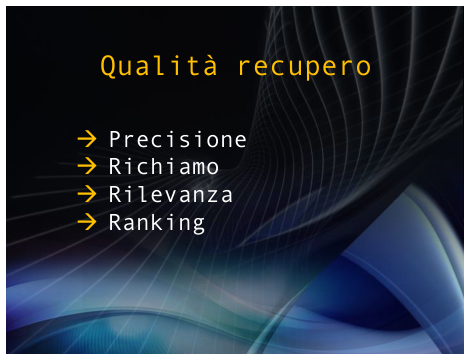
\includegraphics[width=0.50\textwidth,
                    trim=40 100 20 40, % L B R T
                    clip]
                    {images/Lez04_p03_fig_06}
  % \caption{Sommario}
  % \label{fig:Lez15_p06_fig_02}
\end{figure}
\FloatBarrier
\noindent

Parametri di riferimento per l'information retrieval sono per esempio la qualità del recupero.
La qualità del recupero è misurata con quattro parametri, la precisione, il richiamo, la rilevanza e il ranking.
Vediamoli nello specifico.

\FloatBarrier
\begin{figure}[H]
  \centering
  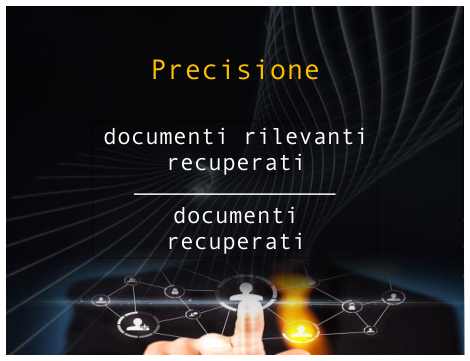
\includegraphics[width=0.50\textwidth,
                    trim=40 100 20 40, % L B R T
                    clip]
                    {images/Lez04_p04_fig_01}
  % \caption{Sommario}
  % \label{fig:Lez15_p06_fig_02}
\end{figure}
\FloatBarrier
\noindent

La precisione è il numero dei documenti rilevanti recuperati, quindi la frazione nell'ambito dei documenti recuperati che ci interessano diviso i documenti recuperati.

\FloatBarrier
\begin{figure}[H]
  \centering
  
\includegraphics[width=0.50\textwidth,
                    trim=40 100 20 40, % L B R T
                    clip]
                    {images/Lez04_p04_fig_02}
  % \caption{Sommario}
  % \label{fig:Lez15_p06_fig_02}
\end{figure}
\FloatBarrier
\noindent

Il richiamo invece ci dà un riferimento dei documenti rilevanti recuperati rispetto all'intera quantità di documenti rilevanti nell'archivio ma che ahimè non sono stati recuperati, perché l'interrogazione non era precisa, non era comprensiva, non era esaustiva e perché la ricerca o l'indicizzazione non hanno permesso la risoluzione esaustiva dell'interrogazione stessa.

\FloatBarrier
\begin{figure}[H]
  \centering
  
\includegraphics[width=0.50\textwidth,
                    trim=40 120 20 40, % L B R T
                    clip]
                    {images/Lez04_p04_fig_03}
  % \caption{Sommario}
  % \label{fig:Lez15_p06_fig_02}
\end{figure}
\FloatBarrier
\noindent

La rilevanza è un elemento, un parametro molto soggettivo.
Può riferirsi sia all'aggiornamento dell'informazione recuperata, cioè al fatto che l'informazione sia in una sua ultima versione, sia autorevole, quindi sia di qualità o sia prodotta da un ente o da una persona di riferimento, o perché l'informazione è innovativa, ci porta qualcosa di nuovo o è di impatto per l'attività che stiamo svolgendo.

\FloatBarrier
\begin{figure}[H]
  \centering
  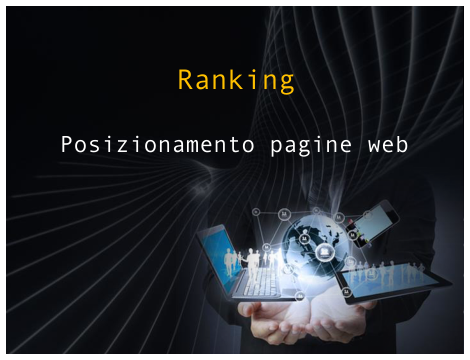
\includegraphics[width=0.50\textwidth,
                    trim=40 140 20 40, % L B R T
                    clip]
                    {images/Lez04_p04_fig_04}
  % \caption{Sommario}
  % \label{fig:Lez15_p06_fig_02}
\end{figure}
\FloatBarrier
\noindent

L'ultimo parametro è il ranking.
Il ranking è un parametro che è stato introdotto in riferimento soprattutto alle pagine web.
Si riferisce proprio al posizionamento delle pagine web rispetto alla navigazione, rispetto alla frequentazione da parte dei cybernavigatori.

\FloatBarrier
\begin{figure}[H]
  \centering
  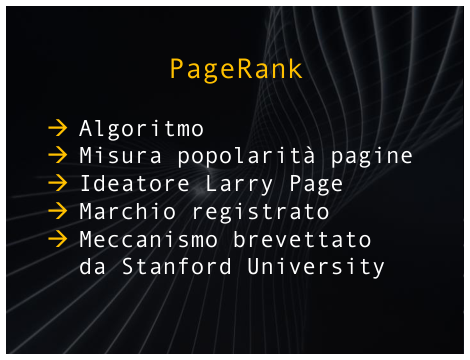
\includegraphics[width=0.50\textwidth,
                    trim=40 80 20 40, % L B R T
                    clip]
                    {images/Lez04_p04_fig_05}
  % \caption{Sommario}
  % \label{fig:Lez15_p06_fig_02}
\end{figure}
\FloatBarrier
\noindent

Il ranking è misurato da un algoritmo che si chiama PageRank.
Misura la popolarità delle pagine web, è un algoritmo che è stato ideato e ha dato il nome Larry Page.
Questo algoritmo è registrato, quindi è un algoritmo molto conosciuto, è diventato uno strumento di riferimento, ma è un marchio che è stato registrato.
L'algoritmo che è stato ideato, il meccanismo che è stato ideato e l'algoritmo che sottostà alla valutazione del PageRank è stato brevetato dalla Università di Stanford dove Larry Page ha iniziato il lavoro su questo strumento.


\subsection{Base di dati}

\FloatBarrier
\begin{figure}[H]
  \centering
  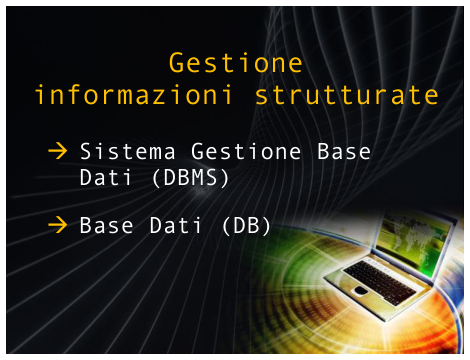
\includegraphics[width=0.50\textwidth,
                    trim=20 80 20 40, % L B R T
                    clip]
                    {images/Lez04_p04_fig_06}
  % \caption{Sommario}
  % \label{fig:Lez15_p06_fig_02}
\end{figure}
\FloatBarrier
\noindent

Passiamo adesso al terzo tipo di un'informazione strutturata quelle che vengono comunemente chiamate base di dati.
Dobbiamo considerare due elementi, i sistemi per la gestione della base di dati e la base di dati.
I sistemi per la gestione della base di dati sono gli insiemi degli strumenti, dei programmi che servono per gestire una base di dati, che è la parte statica, cioè i dati che vengono organizzati, strutturati, rappresentati in una certa maniera.

\FloatBarrier
\begin{figure}[H]
  \centering
  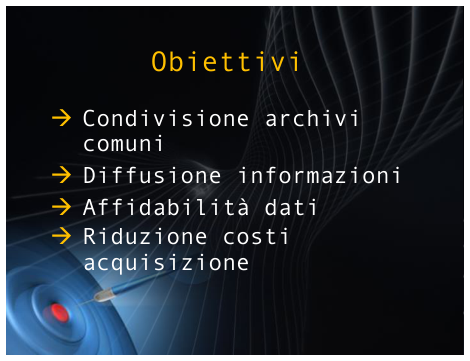
\includegraphics[width=0.50\textwidth,
                    trim=20 80 20 40, % L B R T
                    clip]
                    {images/Lez04_p05_fig_01}
  % \caption{Sommario}
  % \label{fig:Lez15_p06_fig_02}
\end{figure}
\FloatBarrier
\noindent

Obiettivi di un database management system sono la condivisione di archivi comuni, la diffusione delle informazioni, quindi permettere sia a molti utenti di accedere alle informazioni, sia adesso molti archivi sono realizzati online, quindi consultabili anche da postazioni remote, da una vasta categoria di utenti, e permettono anche una rapida e efficiente raccolta di informazioni e quindi una più frequente distribuzione.

I dati che devono essere affidabili, quindi corretti, quindi non duplicati, quindi di riferimento, autorevoli, cioè i dati non devono presentare valori differenti in varie parti dell'archivio che ne mettano in dubbio la correttezza o la congruità.
Infine un obiettivo dell'organizzazione in base di dati è la riduzione dei costi per l'acquisizione di queste informazioni.

\FloatBarrier
\begin{figure}[H]
  \centering
  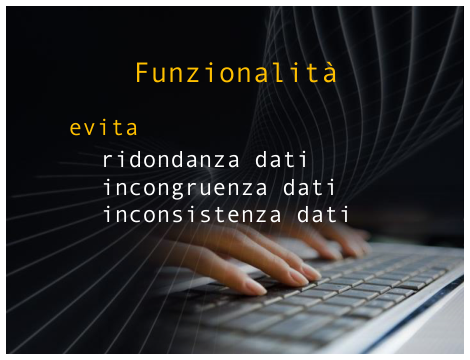
\includegraphics[width=0.50\textwidth,
                    trim=20 80 20 40, % L B R T
                    clip]
                    {images/Lez04_p05_fig_02}
  % \caption{Sommario}
  % \label{fig:Lez15_p06_fig_02}
\end{figure}
\FloatBarrier
\noindent

Le funzionalità di un DBMS.
Evita la ridondanza, quindi la duplicazione dei dati, abbiamo accennato all'incongruenza dei dati, quindi i dati non hanno una unica identificazione nell'ambito degli archivi e l'inconsistenza, i dati presentano varie versioni e non si capisce quale sia, non si riesce più a recuperare quale sia la versione di riferimento.

\FloatBarrier
\begin{figure}[H]
  \centering
  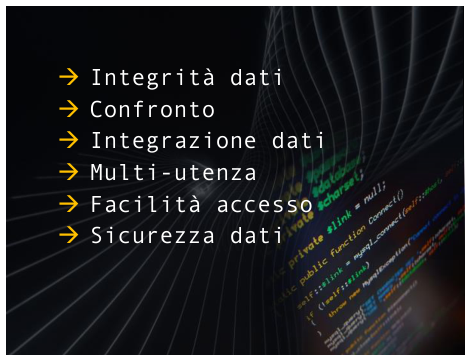
\includegraphics[width=0.50\textwidth,
                    trim=20 80 20 40, % L B R T
                    clip]
                    {images/Lez04_p05_fig_03}
  % \caption{Sommario}
  % \label{fig:Lez15_p06_fig_02}
\end{figure}
\FloatBarrier
\noindent


L'integrità dei dati, che indica che i dati devono essere riferiti costantemente alla definizione che gli ha originati, i dati devono essere confrontabili tra di loro per operazioni o anche per la risoluzione delle interrogazioni.
I dati devono anche essere integrati, quindi un confronto costruttivo, un confronto per produrre nuovi dati o per produrre eventualmente della reportistica basata su statistiche o su confronto su selezioni di dati prodotti con l'aiuto delle basi di dati.

La gestione multiutenti.
In genere una volta che i dati sono costruiti, sono organizzati in base di dati, i costi che sono stati affrontati vengono smaltiti, ammortizzati, permettendo l'uso di questi strumenti a una vasta utenza.
I DBMS forniscono strumenti per la gestione di dati, per il facile accesso a queste basi di dati.
Inoltre, ne proteggono la sicurezza rispetto alla privacy, quindi i dati possono essere protetti da accessi non autorizzati, ma i dati possono essere protetti da eventuali interventi di malintenzionati che ne possono modificare l'autorevolezza.

\FloatBarrier
\begin{figure}[H]
  \centering
  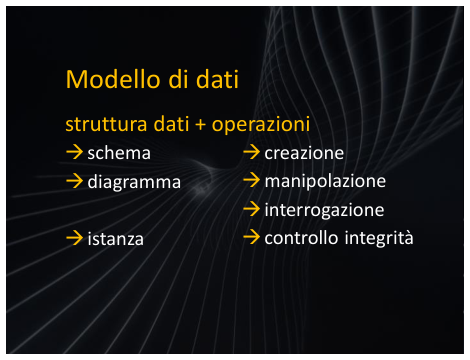
\includegraphics[width=0.50\textwidth,
                    trim=20 80 20 40, % L B R T
                    clip]
                    {images/Lez04_p05_fig_04}
  % \caption{Sommario}
  % \label{fig:Lez15_p06_fig_02}
\end{figure}
\FloatBarrier
\noindent

Nell'organizzazione dei dati sono importanti modelli dei dati.
Modello dei dati è costituito da una struttura più un insieme di operazione.
Allora vediamo a sinistra la struttura di un modello dei dati o di una base di dati è costituita da uno schema che ne definisce la struttura, descrive la struttura che viene mostrata nel diagramma.

Allora il diagramma non è altro che una rappresentazione dello schema.

L'istanza invece è l'insieme dei dati che sono organizzati secondo lo schema.

Le operazioni che vengono fornite da un modello dei dati sono in genere la creazione, quindi la definizione dello schema e del diagramma della base di dati, operazioni per la manipolazione, per l'interrogazione, quindi per la ricerca delle informazioni e per il controllo dell'integrità.

\FloatBarrier
\begin{figure}[H]
  \centering
  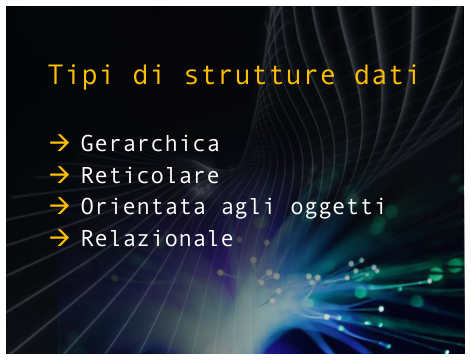
\includegraphics[width=0.50\textwidth,
                    trim=20 80 20 40, % L B R T
                    clip]
                    {images/Lez04_p05_fig_05}
  % \caption{Sommario}
  % \label{fig:Lez15_p06_fig_02}
\end{figure}
\FloatBarrier
\noindent

Vi sono diversi tipi di strutture di dati.
Quella gerarchica in cui i record sono strutturati permettendo l'accesso a più figli, quindi record del livello inferiore, ma ogni record può accedere a livello superiore solo a un altro record.
Questo si esplicita dicendo che ogni record ha un solo padre.

La struttura reticolare invece è analoga alla gerarchica, ma ogni record può avere più padri, quindi ogni record può essere collegato a una quantità arbitraria di record di qualsivoglia livello.

Nelle strutture orientate agli oggetti, gli oggetti sono sostanzialmente caratterizzate dalla loro proprietà di encapsulamento.
Gli oggetti sono elementi in cui il comportamento, quindi gli attributi che descrivono gli oggetti sono i dati, sono accompagnati dalle funzionalità, chiamate metodi, che possono essere utilizzate per operare su questi dati.

Infine la struttura relazionale che è decisamente la struttura più diffusa e organizza ai dati, struttura ai dati su base tabellare.

\FloatBarrier
\begin{figure}[H]
  \centering
  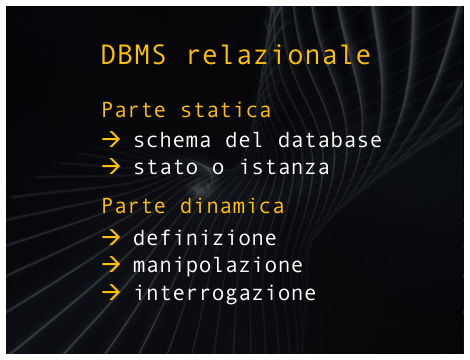
\includegraphics[width=0.50\textwidth,
                    trim=20 80 20 40, % L B R T
                    clip]
                    {images/Lez04_p05_fig_06}
  % \caption{Sommario}
  % \label{fig:Lez15_p06_fig_02}
\end{figure}
\FloatBarrier
\noindent


Un DBMS relazionale è costituito da due parti, una parte statica, quindi lo schema del database e lo stato o istanza del database, cioè i dati che in un dato istante sono archiviati nell'archivio.
E la parte dinamica che è costituita dagli strumenti, dalle operazioni, dai comandi che permettono la definizione dello schema, quindi la definizione della struttura dell'archivio, la manipolazione, quindi l'inserimento, la modifica, la cancellazione dei dati o dello schema stesso e l'interrogazione.
Quindi la possibilità di formulare interrogazioni ma anche la possibilità di risolverle.
I sistemi diciamo di gestione delle basi di dati relazionali forniscono due strumenti per quanto riguarda l'interrogazione.

Un linguaggio di interrogazione che adesso è sostanzialmente l'SQL, è diventato lo standard, structured query language, è lo standard dei linguaggi di interrogazione relazionali.
È stato ideato, definito da COD negli anni 70, nel 79 e offre una sintasi abbastanza semplice, ma per semplificare l'uso del DBMS agli utenti finali viene spesso fornita un'interfaccia grafica o query by example in cui vengono offerti dei template, delle immagini che esemplificano l'organizzazione dei dati che si vuole andare a cercare.

\FloatBarrier
\begin{figure}[H]
  \centering
  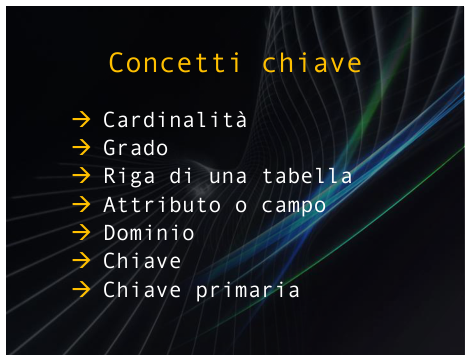
\includegraphics[width=0.50\textwidth,
                    trim=20 80 20 40, % L B R T
                    clip]
                    {images/Lez04_p06_fig_01}
  % \caption{Sommario}
  % \label{fig:Lez15_p06_fig_02}
\end{figure}
\FloatBarrier
\noindent

Vorrei adesso, quasi in conclusione, illustrare alcuni concetti chiave delle basi di dati relazionali.
La cardinalità, abbiamo detto che la base di dati relazionali è un organizzazione di tipo tabellare.
La cardinalità indica il numero delle righe delle tabelle o quelle che vengono chiamate tuple, sequenze di t elementi.
Il grado invece è il numero delle colonne, quindi quanti elementi o quanti attributi definiscono una tabella.
Le righe di una tabella chiamate anche record, tuple, nluple, quindi sequenze di t o n elementi, che sono costituite da n elementi, attributi, chiamati attributi o campi, sono individuati da un nome, ogni colonna di una tabella ha un nome.
Il dominio indica l'insieme dei valori che possono essere assunti dal nome di un attributo o di un campo.

Le chiavi.
La chiave è di due tipi, la chiave generica o chiave esterna ha una funzione di indice per il recupero efficiente delle righe di una tabella, ma anche per il legame tra varie tabelle.
Due chiavi che hanno lo stesso valore in due tabelle differenti, in due relazioni differenti, permettono il collegamento di record che assumono quel valore.

Le chiavi primarie hanno in più la proprietà di essere caratterizzati una tupla, quindi il loro valore è univoco per ogni record.

\FloatBarrier
\begin{figure}[H]
  \centering
  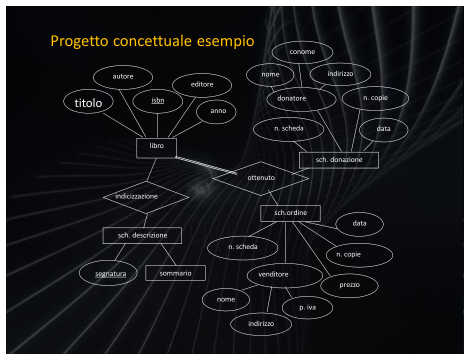
\includegraphics[width=0.50\textwidth,
                    trim=20 20 20 20, % L B R T
                    clip]
                    {images/Lez04_p06_fig_02}
  % \caption{Sommario}
  % \label{fig:Lez15_p06_fig_02}
\end{figure}
\FloatBarrier
\noindent


Il progetto di una base di dati è effettuato a due livelli, in questo caso vedete il livello concettuale, il progetto concettuale di una base di dati viene realizzato utilizzando un modello grafico entity relationship in cui i tipi di entità che vengono rappresentati, un'entità può essere concreta ma anche ideale sono rappresentati da quadrati.
I rombi indicano le relazioni tra i vari tipi.
Gli archi sono ovviamente i legami tra le relazioni e i tipi di entità.
Gli attributi sono indicati con degli ovali.
Il progetto concettuale di alto livello è il primo livello di progetto che è realizzato con l'utente.

\FloatBarrier
\begin{figure}[H]
  \centering
  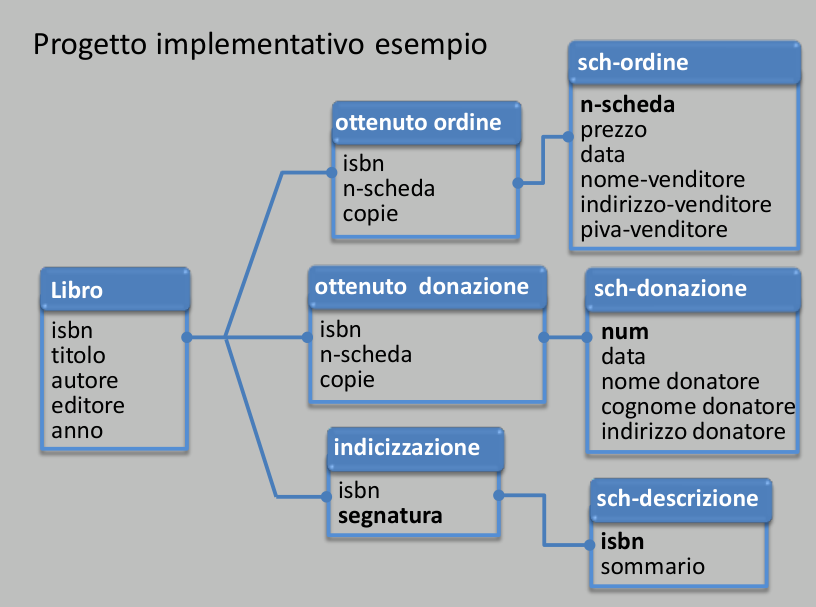
\includegraphics[width=0.50\textwidth,
                    trim=00 00 00 00, % L B R T
                    clip]
                    {images/Lez04_p06_fig_03}
  % \caption{Sommario}
  % \label{fig:Lez15_p06_fig_02}
\end{figure}
\FloatBarrier
\noindent

Viene poi tradotto in tabelle in cui ogni entità o relazione viene rappresentata da tabelle che sono collegate attraverso chiavi che possono essere primarie o esterne.
Alla fine di questo argomento e quindi di questa lezione vi propongo due spunti di riflessione.
Quali tipi di gestione delle informazioni individuate nel vostro ambito lavorativo formativo? Tutte tre? Solo alcuni?
Alcuni sono preponderanti, argomentate.